\chapter{引言}

\section{暗物质研究的意义}
\subsection{暗物质存在的证据}

\subsection{标准模型之外的物理}
现有模型的拓展:SUSY supersymmetry 有暗物质候选粒子

\subsection{实验数据的缺失}

\section{暗物质的空间探测}
暗物质粒子探测是当前的科学热点, 具有重要的物理意义和前景, 因此世界各国都在集中人力、物力和财力研究这一问题。
\subsection{暗物质探测的方法和难点}
根据目前的技术手段, 探测暗物质粒子的方法大致可以总结为三类: 加速器直接产生法, 直接探测法和间接探测法。

加速器直接产生法是发现新粒子最常用和最有效的方法。
利用高能加速器将粒子加速到超高能量进行对撞可以模拟宇宙大爆炸环境, 各种各样新的粒子能够在对撞后产生, 其中也可能包含暗物质候选粒子。
通过对次级粒子的探测或逃逸能量(missing energy)的重建, 可以反推出新粒子的存在并准确研究其物理特性。
产生暗物质候选粒子需要极高的能量(TeV量级), 目前只有欧洲核子中心的大型强子对撞机(LHC)能够满足这个条件。
然而, LHC只能产生较轻的暗物质粒子候选粒子, 对于更重的暗物质候选粒子, 需要建造更高能量的加速器和更加强大的粒子探测器。

第二种是直接探测暗物质粒子。该方法是直接探测来自宇宙空间的暗物质粒子与(探测器上的)原子核碰撞所产生的信号。

第三种间接探测暗物质粒子。间接法是观测暗物质粒子在宇宙空间发生衰变或相互作用之后产生的稳定粒子如伽玛射线、正电子、反质子、中微子等。

\subsection{空间探测的优势}

\subsection{国际上的空间探测项目与研究现状}

\section{DAMPE暗物质粒子探测卫星}

暗物质粒子子探测卫星 (英文: DArk Matter Particle Explorer, 缩写: DAMPE)是
\subsection{物理目标}
%\subsection{工作原理}
\subsection{探测器组成}
\begin{figure}
\centering
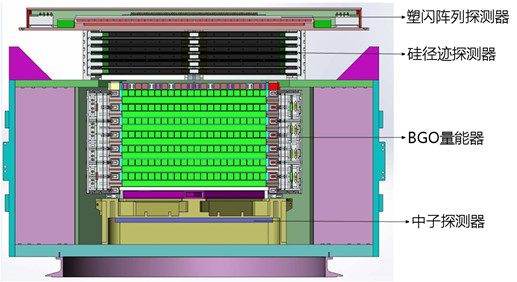
\includegraphics[width=0.9\linewidth]{chap/introduction/fig/dampe_structure_2}
\caption{DAMPE暗物质粒子探测器的整体结构}
\label{fig:dampe_structure}
\end{figure}
